\renewcommand{\chaptername}{Глава}
\chapter{Структура проекта «Тортуга»} \label{chapt1}
Программа «Тортуга» является проектом компании «Образование IT», которая ставит перед собой цель обучение школьников основам программирования. Программа представляет собой Web–приложение, построенное на языке JavaScript, с использованием технологий HTML5 и CSS3. Благодаря применению данных технологий, нет необходимости в постоянном доступе к сети Интернет. Использовать «Тортугу» можно, скопировав на флешку или любой другой цифровой носитель страницу сайта, где расположено данное приложение.\par
Один из сценариев работы с «Тортугой» следующий. Преподаватель на странице constructor.html создает урок: формулирует тексты и название задачи. Информация об уроке особым образом кодируется и формируется ссылка с текстом этого урока, пройдя по которой, откроется страница index.html с текстом задания. Для выполнения задачи ученику потребуется создать объект Черепашка и, управляя ее действиями через команды, достигнуть поставленной задачи.\par
Часто учителям не удается заинтересовать школьников предметом лишь потому, что не могут найти хорошего задания. По этому в «Тортуге» любой человек может самостоятельно построить именно такой урок, который будет ему необходим, что важно для применения в школах. Вариант готового урока можно увидеть на рис. 1. 
\vspace{50mm}

\begin{figure} [h] 
  \center
  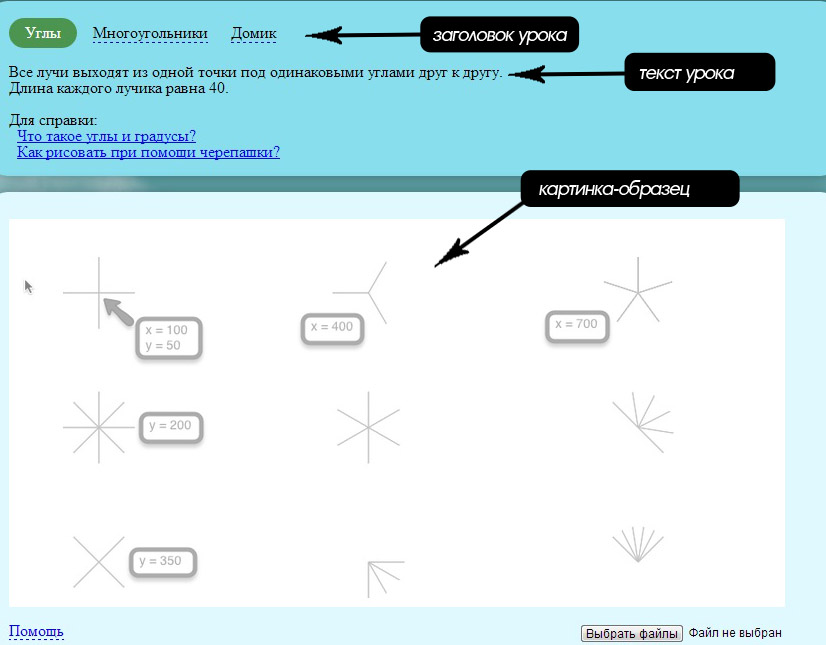
\includegraphics [scale=0.70,natwidth=826,natheight=645] {images/pic1.jpg}
  \caption{Пример урока.} 
  \label{img:pic1}  
\end{figure}


Для создания урока на странице constructor.html в текстовое окно вводится текст урока и, при нажатии кнопки «Создать», содержимое текстового поля извлекается, сжимается, кодируется base64 и создается ссылка на урок.\par
Процесс разработки «Тортуги» ориентирован на то, чтобы программа работала в последних версиях Chrome и Яндекс браузер. Но на данный момент работает и в Fierfox, Safari, IE 8+, Opera, но при возникновении проблем поддержка этих браузеров осуществляется по остаточному принципу.\par
% % % % % % % % % % % % % % % % % % % % % % % % % % % % % % %
\chapter{Сокращение ссылки} \label{chapt1}

Как было сказано выше, сценарий работы с «Тортугой» – это работа с приготовленными уроками, которые открываются по ссылке вида: \par
\vspace{6mm}
\begin{center}
 \textit{ http://tortuga/index.html?b4/wMsYxLAwL/+Ml5/HjEw } (1)\par

\end{center}
\vspace{6mm}

Урок содержит тексты задачи, ссылки на картинки–обазцы, поэтому ссылка получается довольно длинной, например: \par

\begin{center}
\vspace{6mm}
 \textit{ http://tortuga/index.html?7VcxTkMxDL2K9eeqB+gMGys
 TZTCJWywlTkhshIS4O04LN2AA5O3nx35+fk+OkvdNWQ
 tth+2uDarAfVqF3EobMFkBK+kOUpNJSUltAGbuPDmxn
 IEK++6k7BlAbLO2fBSl2j2dJXHmbKJgCgWfvACQXsEJ
 Kp4FAQu/GO7hXoGEq6ND5fXx6kusu6O8GE+QNnVYBnq
 jkVhRuQlYKVhTu0KvIKe1Sl0wuXswEDr36qzaUS5NeD
 Hdw83CRFMCHuZcrv2ywKA+6Jkk0/Dm/cdrK9a9Hjkhb
 xZoTnIoLuVbJu/J4GRnRgVZlKDj8IWNPdy+JepKtrRG
 VpKSMnjknXOqCujyVH6aJxJlpRLLS+brHQE7wLa6eRa
 I2SaNNZubWURwSUSuyLzS1ur+7Dwz1u47TZ28ed2eHi
 P0fxXvs6Rwss4ZsPCsDAs/JET1cPS4L70iZM1xjIs/A
 1j+bGLi2uMZFgYb4/wMsYxLAwL/+Ml5/HjEw== } (2)\par
\end{center}

\vspace{6mm}

Делиться ссылкой такого размера, отправлять по почте, размещать в соц–сетях, использовать в презентациях весьма неудобно. В связи с чем появилась необходимость укорачивания ссылки до 20 знаков и менее. Уже довольно давно существуют способы их сокращения при помощи сайтов–сокращателей таких как:  \textit{www.bitly.com, www.gg.gg, www.goo.gl} и др. Необходимо зайти на соответствующую страницу и после ввода в текстовое окно длинной ссылки, создастся короткая, вида:
 
\begin{center}
\vspace{6mm}
 \textit{ http://goo.gl/fbsS } (3)\par
\end{center}

при переходе по которой происходит перенаправление на длинную. Но такое ручное использование удобно только для единичных вариантов. Что бы создателю уроков не приходилось каждый раз выполнять все эти рутинные операции, возникла задача автоматизировать процесс сокращения ссылок. Для этого было решено воспользоваться API, которое предоставляет Google. Была найдена и использована сторонняя библиотека Jsonlib ~\cite{jsonlib} (автор Девид Бау/David Bau). С ее помощью можно обмениваться запросами в формате JSON технологией AJAX не напрямую, а через сторонний сервер, который осуществляет обращения и возвращает ответ. В связи с чем были созданы функции \textit{getShortenURL} и \textit{parseShortenedResponse}. Одна из которых отправляет запрос с передачей длинной ссылки, а вторая, получив ответ в формате JSON, и, распарсив, выводит на страницу constructor.html в текстовое окно. Если по какой-либо причине запрос не был осуществлен или ответ не был получен, на страницу выводится  длинный URL (см. приложение \ref{AppendixA3} ).


% % % % % % % % % % % % % % % % % % % % % % % % % % % % % % %
\chapter{Очистка экрана} \label{chapt1}
При выполнении урока ошибки в алгоритмах рисования неизбежны, и единственный способ очистки экрана - это обновление страницы. Но сраница долго перегружается и приходится заново создавать черепаху с соответствующими настройками положения на экране, ее цветом и толщиной рисования, что отвлекает и создает неудобства. Решением проблемы была бы возможность очистки экрана без обновления страницы. Для этого в библиотеку функций была добавлена еще одна публичная функция \textit{clearCanvas()}, очищающая прямоугольник размером с Canvas (см. приложение \ref{AppendixA3}). Помимо решения такой проблемы очистка экрана дает дополнительные возможности в программировании, например создание анимации.

% % % % % % % % % % % % % % % % % % % % % % % % % % % % % % %
\chapter{Изменение толщины рисования} \label{chapt1}

Дополнительное разнообразие достигается при возможности изменения толщины рисования черепахи. Для реализации этого функционала в объект, представляющий черепаху, добавлено свойство width, а в прототип (объект, представляющий свойства и методы, общие для всех черепах) была добавлена функция \textit{setWidth}, внутри которой передаваемая в качестве параметра толщина присваивается конкретной черепахе. Так как доступ к графическому объекту Canvas доступен через графические методы, с помощью которых манипуляции с черепахой отражаются на Canvas, то добавлена открытая функция \textit{setWidth} (см.приложение \ref{AppendixA3}) ~\cite{prototype}.

% % % % % % % % % % % % % % % % % % % % % % % % % % % % % % %
\chapter{Изменение толщины рисования} \label{chapt1}

Во время использования созданных уроков возможно выявление  неточностей, ошибок в орфографии и других недочетов, которые требуют исправления. Для этого функционал приложения был дополнен инструментом для редактирования уроков. Для его создания на страницу создания уроков \textit{constructor.html} было добавлено текстовое поле \textit{lessonInput}, в которое вставляется ссылка на уже имеющийся урок. При нажатии на кнопку «Изменить урок» данные из \textit{lessonInput} передаются в свойство \textit{givLessonArea} объекта Tortuga для вызова закрытой функции \textit{updateArea}, которая, в свою очередь,  извлекает текст из ссылки, разархивирует, парсит, и вставляет в текстовое окно в том виде, в котором он был введен. После чего текст урока можно править и далее, при нажатии кнопки «создать урок», формируется новая ссылка на исправленный урок. (см. приложение \ref{AppendixA3}) ~\cite{elementsdom, string}.

% % % % % % % % % % % % % % % % % % % % % % % % % % % % % % %


%\newpage
%============================================================================================================================

\clearpage